\documentclass[a4paper, amsfonts, amssymb, amsmath, reprint, showkeys, nofootinbib, twoside]{revtex4-1}
\usepackage[spanish]{babel}
\usepackage[utf8]{inputenc}
\usepackage{float}
\usepackage[colorinlistoftodos, color=green!40, prependcaption]{todonotes}
\usepackage{amsthm}
\usepackage{mathtools}
\usepackage{physics}
\usepackage{xcolor}
\usepackage{graphicx}
\usepackage[left=23mm,right=13mm,top=35mm,columnsep=15pt]{geometry} 
\usepackage{adjustbox}
\usepackage{placeins}
\usepackage[T1]{fontenc}
\usepackage{lipsum}
\usepackage{tikz}
\usepackage{circuitikz}
\usepackage{csquotes}
\usepackage[normalem]{ulem}
\useunder{\uline}{\ul}{}
\usepackage[pdftex, pdftitle={Article}, pdfauthor={Author}]{hyperref} % For hyperlinks in the PDF
%\setlength{\marginparwidth}{2.5cm}
\bibliographystyle{apsrev4-1}

\begin{document}

%El título del experimento realizado es importante.
\title{Analisis de circuitos resistivos. Manejo de multimetro (Preinforme Sesión 1)}


\author{Sergio Montoya Ramirez}
\email[Correo institucional: ]{s.montoyar2@uniandes.edu.co}

%Si necesitan poner un segundo autor, deben eliminar los porcentajes (%) iniciales.
  
%\author{Second Author}
%\email{Second.Author@institution.edu}

\affiliation{Universidad de los Andes, Bogotá, Colombia.}

\date{\today} % Si lo dejan vacío no les saldrá fecha. La fecha que se muestra es del día en que se compila.

\begin{abstract}

  Este texto es el preinforme de la sesión 1 del experimento 3 del curso Electronica para Ciencias de la Universidad de los Andes durante el semestre 202310. Tiene como objetivo la preparación para el posterior desarrollo de la sesión previamente enunciada.

\end{abstract}

\maketitle

\begin{figure}[h]
  \centering
  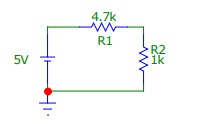
\includegraphics[width=0.4\textwidth]{Graficas/Circuito1.jpeg}
  \caption{Grafica del divisor de voltaje}
  \label{fig:divisor_voltaje}
\end{figure}	

\begin{figure}[h]
  \centering
  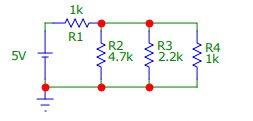
\includegraphics[width=0.4\textwidth]{Graficas/Circuito2.jpeg}
  \caption{Grafica del divisor de corriente}
  \label{fig:divisor_corriente}
\end{figure}

\section{Identificación de Mallas y Nodos}

Para cada circuito en las figuras \ref{fig:divisor_voltaje} y \ref{fig:divisor_corriente} identifique y señale cada posible malla y nodo existente.

\begin{enumerate}
  \item \textbf{Divisor de Voltaje}
    \begin{enumerate}
      \item \textit{Nodos:}

	En este caso tenemos 3 nodos. El que esta entre la fuente y la resistencia de $4.7k$, El que esta entre las dos resistencias y el que se eligio como polo a tierra.
	
      \item \textit{Mallas:}

	En este caso tenemos una sola malla que es aquella que recorre todos los componentes del circuito.
    \end{enumerate}
  \item \textbf{Divisor de Corriente}
    \begin{enumerate}
      \item \textit{Nodos:}

	En este caso tenemos 3 nodos, El nodo entre la fuente y la resistencia de $1k$. El nodo entre $R_1,R_2,R_3,R_4$. y el que se identifica como polo a tierra.

      \item \textit{Mallas:}

	En este caso tenemos 6 mallas. Las tres mallas internas, las mallas que juntan dos mallas internas, es decir derecha-centro y centro-izquierda y por ultimo la malla exterior. cada una de estas mallas pasa por los siguientes componentes:
	\begin{enumerate}
	  \item Fuente,$R_1$,$R_2$ 
	  \item $R_2$,$R_3$ 
	  \item $R_3$,$R_4$ 
	  \item Fuente, $R_1$,$R_3$ 
	  \item $R_2$, $R_4$
	  \item Fuente, $R_1$, $R_4$ 
	\end{enumerate}
    \end{enumerate}
\end{enumerate}

\section{Leyes de Kirchhoff}

Para cada circuito, usando el metodo de leyes de Kirchhoff de su elección calcule la corriente y voltaje a través de cada resistencia.

\begin{enumerate}
  \item \textbf{Divisor de Voltaje:} 

    Para este circuito vamos a utilizar ley de nodos. En este caso, por el nodo que esta entre las dos resistencias sabemos que:
    \begin{equation*}
      I_1 = I_2
    \end{equation*}
    
    En cuyo caso, para $I_1$ e $I_2$ por ley de Ohm queda:
    \begin{align*}
      I_1&=\frac{v_{f}-v_{x}}{R_{1}} \\
      I_{2} &= \frac{v_x - 0}{R_2}
    .\end{align*}

    Ahora una vez mas si utilizamos que $I_1=I_2$ nos queda:
    \begin{align*}
      I_1&= I_2 \\
      \frac{v_f - v_x}{R_1}&= \frac{v_x - 0}{R_2} \\
      \frac{v_f}{R_1}&= \frac{v_x}{R_2} + \frac{v_2}{R_1} \\
      \frac{v_f}{R_1} &= v_x \frac{R_2+R_1}{R_2R_1} \\
      v_f \frac{R_2}{R_2+R_1} &= v_x \\
      v_x &= 5 \frac{1k}{4.7k + 1k}\\
      &= \frac{5k}{5.7k}
    .\end{align*}

  \item \textbf{Divisor de Corriente:}

    En este caso, utilizaremos ley de nodos para realizar este trabajo.
    \begin{align*}
      I_1 &= I_2 \\
      I_2 &= I_3 + I_4 + I_5 \\
      I_3 + I_4 + I_5 &= I_1 \\
      V_c &= 0 \\
      V_a - V_c &= 5v \\
      V_a - V_b &= I_2R_1 \\
      V_b - V_c	&= I_3R_{2} \\
      V_b - V_c &= I_4R_3 \\
      V_b - V_c &= I_5R_4 \\
    .\end{align*}

    Con esto entonces podemos ahora si reducir ecuaciones de manera que nos quede:
    \begin{align*}
      I_4 &= \frac{R_2}{R_3}I_3 \\
      I_5 &= \frac{R_2}{R_4}I_3 \\
      I_2 &= I_3+I_4+I_5 \\
      I_2 &= I_3\left( 1 + \frac{R_2}{R_3}+\frac{R_2}{R_4} \right)  \\
      &= R_2I_3\left( \frac{1}{R_2}+\frac{1}{R_3}+\frac{1}{R_4} \right)  \\
      I_3R_2 &= 5V - R_1R_2I_3\left( \frac{1}{R_2}+\frac{1}{R_3}+\frac{1}{R_4} \right)  \\
      5V &= I_3\left[ R_2+R_1R_2\left( \frac{1}{R_2}+\frac{1}{R_3}+\frac{1}{R_4} \right)  \right] \\
      I_3 &= \frac{5V}{R_2+R_1R_2\left( R_2+R_3+R_4 \right) }
    .\end{align*}

    Que ahora solo nos faltaria calcular numericamente
    \begin{align*}
      I_1&= I_2=3.13mA \\
      I_3 &= 0.40 mA \\
      I_4 &= 0.85mA \\
      I_5 &= 1.88mA \\
      V_a &= 5V\\
      V_b &= 1.88V \\
      V_c &= 0
    .\end{align*}

\end{enumerate}

\section{Conversión Fuentes}

Para el circuito de la figura \ref{fig:divisor_corriente} transforme la fuente de voltaje en serie con la resistencia de $1k\Omega$ por una fuente de corriente en paralelo con una resistencia. Para este nuevo circuito calcule la corriente y el voltaje a travez de cada resistencia.

En este caso tenemos que el circuito que queda es:
 \begin{circuitikz}
      \draw (0,0)
      to[V,v=$I_f$] (0,2) % The voltage source
      to[short] (2,2)
      to[R=$R_1$] (2,0) % The resistor
      to[short] (0,0);
      \draw (2,2)
      to[short] (4,2)
      to[R=$R_2$] (4,0)
      to[short] (2,0);
      \draw (4,2)
      to[short] (6,2)
      to[R=$R_3$] (6,0)
      to[short] (4,0);
      \draw (6,2)
      to[short] (8,2)
      to[R=$R_4$] (8,0)
      to[short] (6,0);
   \end{circuitikz}

   donde $5V=I_f\cdot R_1$
   
   Y ahora resolvemos por mallas.
   \begin{align*}
     M_1&: I_f=I_1\\
     M_2&: 0=\left( I_2-I_1 \right) R_1 + \left( I_2-I_3 \right) R_2\\
     M_3&: 0=\left( I_3-I_2 \right) R_2 + \left( I_3+I_4 \right) R_3 \\
     M_4&: 0=\left( I_4-I_3 \right) R_3 + I_4R_4
   .\end{align*}

   En este caso lo podemos reescribir como:
   \begin{align*}
     \begin{pmatrix} R_1+R_2 & -R_2 & 0 \\
       -R_2 & R_2+R_1 & -R_{3}\\
       0 & -R_1 & R_4
     \end{pmatrix} \begin{pmatrix} I_2\\ I_3 \\ I_4 \end{pmatrix} = \begin{pmatrix} I_1R_1 \\ 0 \\ 0 \end{pmatrix} \\
     \begin{pmatrix} I_2\\I_3\\I_4 \end{pmatrix} = \begin{pmatrix} 3.13\\2.73\\1.88 \end{pmatrix} 
   .\end{align*}

   \section{Notas sobre la realización}

   Para el desarrollo de este trabajo se utilizo por un lado las diapositivas de la clase magistral: \textit{Diapositivas 2: Analisis de Circuitos} y por el otro se le solicito ayuda a un compañéro.
\end{document}
